\begin{figure}[htbp]
  \centering
  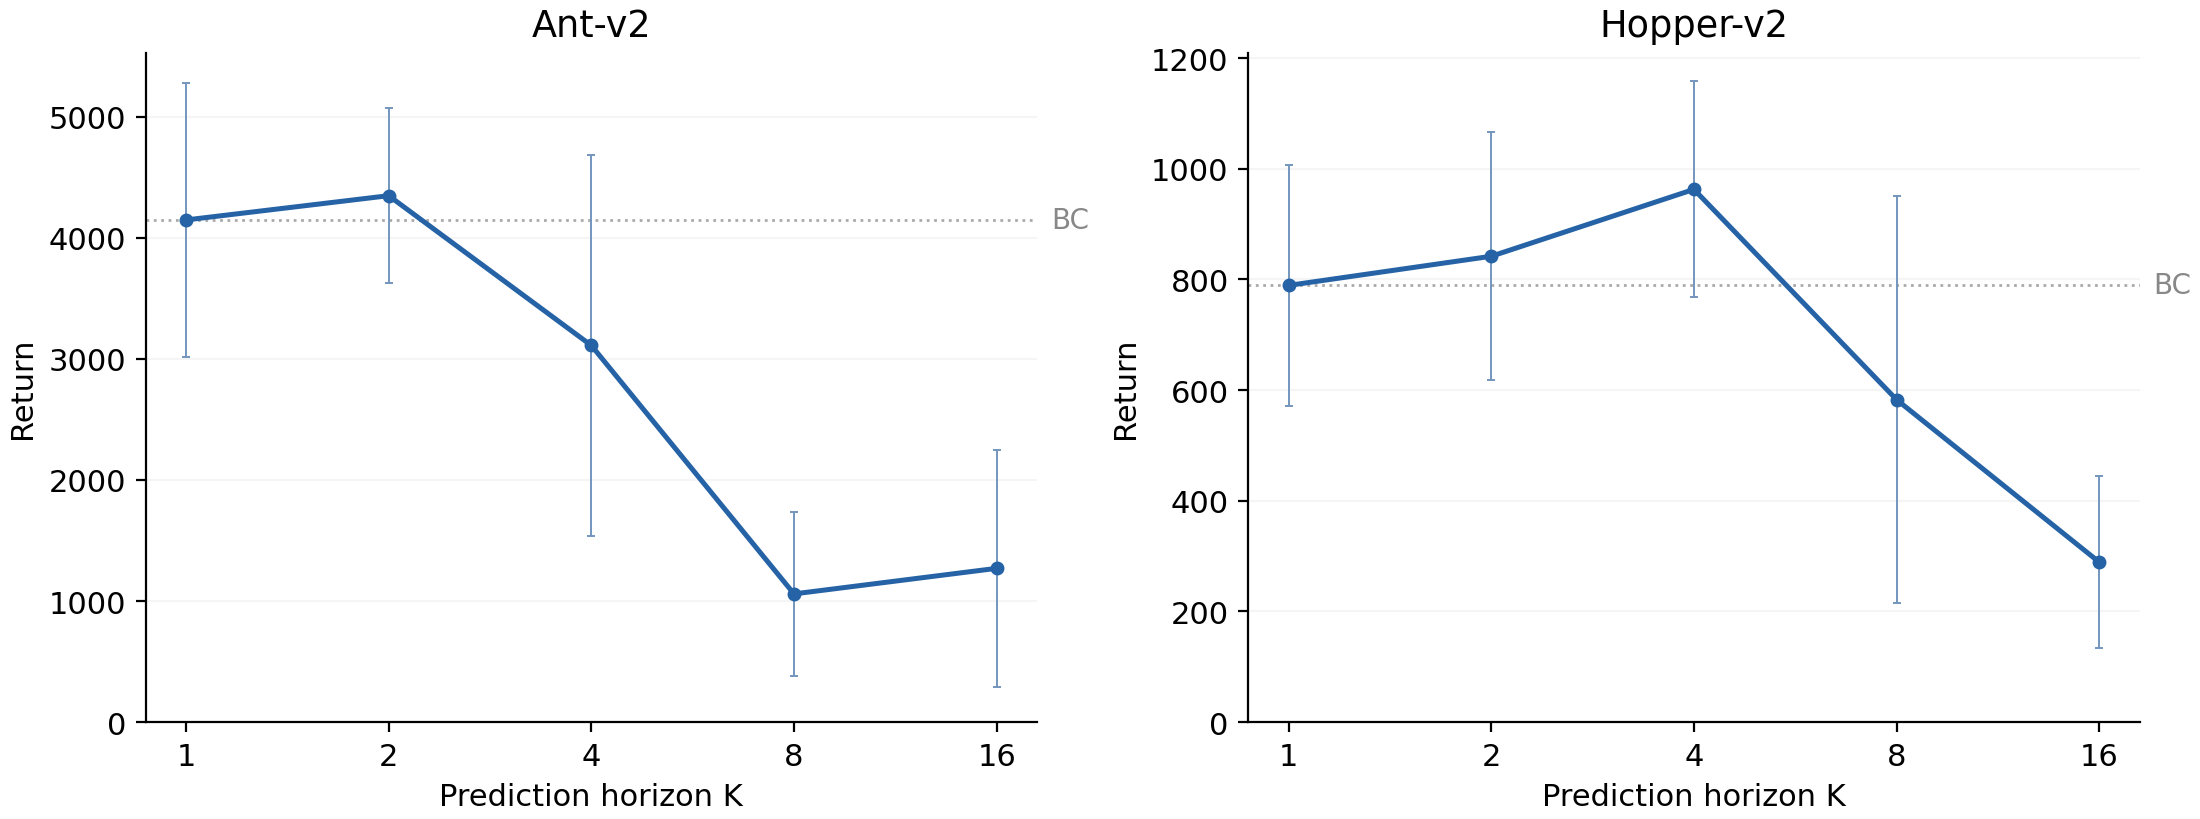
\includegraphics[width=\linewidth]{../results/action_chunks/ant_hopper/figure1.png}
  \caption{Effect of action-prediction horizon on BC in Ant-v2, Hopper-v2. Hypothesis: predicting future expert actions can improve imitation by providing temporal supervision. We vary $K\in\{1,2,4,8,16\}$ and minimize MSE averaged over valid action offsets; $K=1$ is classic BC; dotted lines show its mean return in this sweep. Only the first predicted action is executed, with replanning every step. Within each task, all conditions use the same two demonstrations (2,000 starting observations), 3 hidden layers of 64 tanh units, Adam with learning rate 0.005, 1000 updates, and minibatches of 100. Hidden layers and the current-action output are initialized identically per seed; missing tail targets are masked. Each of 3 training seeds is evaluated on the same 20 reset seeds across horizons, with an episode limit of 1000 steps. Points and bars show mean and population standard deviation over 60 episode returns, not confidence intervals. Ant-v2: K=2 exceeded the classic BC mean, providing limited descriptive support for the hypothesis; this is not a significance result. Hopper-v2: K=2, 4 exceeded the classic BC mean, providing limited descriptive support for the hypothesis; this is not a significance result.}
  \label{fig:p4}
\end{figure}
